\documentclass[11pt]{article}

\usepackage[utf8]{inputenc}
\usepackage[margin=1in]{geometry} 
\usepackage{amsmath,amsthm,amssymb,graphicx,mathtools,tikz,hyperref,multicol,cancel,enumitem,booktabs,float,pgfplots,multirow,mathrsfs,textcomp,gensymb,soul,changepage,threeparttable}
%\usepackage[table]{xcolor}
\usepackage[T1]{fontenc}
\usepackage{subfig}
\usepackage[italian]{babel}
\usepackage{hyphenat}
\hyphenation{mate-mati-ca recu-perare}
\usetikzlibrary{positioning}
\pgfplotsset{compat=1.14}

\newcommand{\n}{\mathbb{N}}
\newcommand{\z}{\mathbb{Z}}
\newcommand{\q}{\mathbb{Q}}
\newcommand{\cx}{\mathbb{C}}
\newcommand{\real}{\mathbb{R}}
\newcommand{\field}{\mathbb{F}}
\newcommand{\ita}[1]{\textit{#1}}
\newcommand{\com}[2]{#1\backslash#2}
\newcommand{\oneton}{\{1,2,3,...,n\}}
\newcommand{\idea}[1]{\begin{gather*}#1\end{gather*}}
\newcommand{\ef}{\ita{f} }
\newcommand{\eff}{\ita{f}}
\newcommand{\proofs}[1]{\begin{proof}#1\end{proof}}
\newcommand{\inv}[1]{#1^{-1}}
\newcommand{\setb}[1]{\{#1\}}
\newcommand{\en}{\ita{n }}
\newcommand{\vbrack}[1]{\langle #1\rangle}
\newcommand{\qRa}{\quad \Rightarrow \quad}
\newcommand{\smaca}[1]{\textbf{\textsc{#1}}}

\newenvironment{theorem}[2][Teorema]{\begin{trivlist}
\item[\hskip \labelsep {\bfseries #1}\hskip \labelsep {\bfseries #2.}]}{\end{trivlist}}
\newenvironment{lemma}[2][Lemma]{\begin{trivlist}
\item[\hskip \labelsep {\bfseries #1}\hskip \labelsep {\bfseries #2.}]}{\end{trivlist}}
\newenvironment{exercise}[2][Esercizio]{\begin{trivlist}
\item[\hskip \labelsep {\bfseries #1}\hskip \labelsep {\bfseries #2.}]}{\end{trivlist}}
\newenvironment{proposition}[2][Proposizione]{\begin{trivlist}
\item[\hskip \labelsep {\bfseries #1}\hskip \labelsep {\bfseries #2.}]}{\end{trivlist}}
\newenvironment{corollary}[2][Corollario]{\begin{trivlist}
\item[\hskip \labelsep {\bfseries #1}\hskip \labelsep {\bfseries #2.}]}{\end{trivlist}}

\hypersetup {
    colorlinks,
    linkcolor=blue
}

\graphicspath{{img/}}

\begin{document}
\setlength{\parindent}{0pt}
\title{\vspace{-4em}{\large Laboratorio di Meccanica e Termodinamica} \\
    Relazione di Laboratorio}
\author{GRUPPO 3 \\
        Gerardo Selce, Maurizio Liguori, Emanuela Galluccio, Francesco Messano}
\date{19/11/2024}
\maketitle

\vspace{-2em}\par\noindent\rule{\textwidth}{0.4pt}
\begin{center}
    {\Large\sc Determinazione della costante elastica della molla}  
\end{center}
\par\noindent\rule{\textwidth}{0.4pt}

%%%%%%%%%%%%%%%%%%%%%%%%%%%%%%%%%%%%%%%%%%%%%%%%%%
% INTRODUZIONE
%%%%%%%%%%%%%%%%%%%%%%%%%%%%%%%%%%%%%%%%%%%%%%%%%%
\section{Introduzione}

É assegnata una molla con costante elastica $k$ ignota. Scopo dell'esperienza è la determinazione della costante $k$ attraverso due approcci, denominati rispettivamente \textbf{metodo statico} e \textbf{dinamico}. Nel primo caso (metodo statico) la molla, sospesa verticalmente su un supporto, è stata sottoposta a carichi crescenti applicando masse in modo progressivo e lineare.
Per non compromettere le caratteristiche strutturali della molla, sono state utilizzate masse tali da causare allungamenti inferiori al doppio della sua lunghezza a riposo. Per ciascun valore della massa applicata, è stata registrata la corrispondente variazione di lunghezza rispetto alla condizione iniziale di riposo. Graficando tali lunghezze in funzione delle masse si ricava una prima stima del valore di $k$, sfruttando la legge:
\begin{equation}
    Mg = k\Delta x
\end{equation}
Nel secondo caso (metodo dinamico) è stato misurato il periodo di oscillazione della molla per ognuna delle masse utilizzate nella prima parte. Infine, ricorrendo alla seguente legge:
\begin{equation}
    T = 2\pi \sqrt{\frac{M}{k}}
\end{equation}
è stata ricavata una seconda stima per $k$, successivamente confrontata con la prima stima per verificare la coerenza dei risultati ottenuti.

%%%%%%%%%%%%%%%%%%%%%%%%%%%%%%%%%%%%%%%%%%%%%%%%%%
% RICHIAMI TEORICI
%%%%%%%%%%%%%%%%%%%%%%%%%%%%%%%%%%%%%%%%%%%%%%%%%%
\section{Richiami teorici}
Il funzionamento del sistema massa-molla si basa sulla Legge di Hooke, la quale stabilisce che la deformazione elastica di un materiale è direttamente proporzionale alla forza applicata, a condizione che tale deformazione non superi un valore critico, detto \textbf{limite elastico} della molla. La legge di Hooke si può esprimere al seguente modo:
\begin{equation}
    \vec{F'} = k\Delta\vec{x}
\end{equation}
Dove:
\begin{itemize}
    \item $\vec{F}$: Forza applicata $[N]$.
    \item k: Costante elastica della molla $[\frac{N}{m}]$.
    \item $\Delta\vec{x}$: Allungamento (o compressione) della molla rispetto alla posizione di equilibrio $[m]$.
\end{itemize}
Pertanto, per il terzo principio della dinamica, la forza esercitata dalla molla su una massa $m$ applicata sarà pari ad $\vec{F} = -\vec{F'}$. La legge è valida solo entro il limite elastico della molla, in cui il sistema è in grado di ritornare alla sua forma originale, una volta rimossa la forza. Superato tale limite, si entra nel campo plastico o nei casi più estremi, si arriva alla rottura del materiale. Per un sistema massa-molla disposto verticalmente come nel nostro caso, in condizioni ideali (trascurando la massa della molla e la forza di attrito esercitata dall'aria) le uniche forze in gioco sono la forza peso $\vec{F}_g$ e la forza elastica $\vec{F}$ esercitata dalla molla. Entrambe le forze agiscono lungo la verticale. Fissiamo perciò un asse verticale orientato concordemente alla forza peso, che è sufficiente per descrivere l'evoluzione dinamica del sistema, poichè le forze agenti hanno componenti nulle su qualsiasi altro asse perpendicolare a quello scelto. 
\begin{figure}[H]
  \centering
  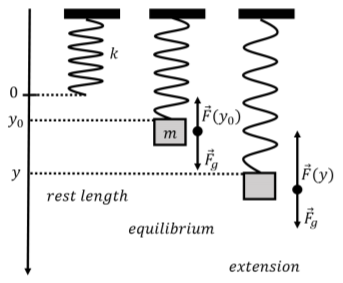
\includegraphics[width=0.45\textwidth]{sistema_massa_molla.png}
  \caption{sistema massa-molla verticale.}
\end{figure}
Fissiamo l'origine degli assi nel punto corrispondente alla posizione dell'estremo libero della molla a riposo. Quando a questo viene attaccata la massa $m$, la molla subisce una deformazione che porta $m$ in una nuova posizione di equilibrio $y_0$.
\subsection{Metodo Statico}
Dalla seconda legge di Newton, proiettata sull'asse di riferimento, si ottiene, per la nuova posizione di equilibrio:

\begin{align}
    F_g - F(y_0) &= 0 \\
    mg - ky_0 &= 0 \\
    mg &= ky_0
\end{align}
Otteniamo così la Legge (1).

\subsection{Metodo Dinamico}
Applicando ora la legge di Newton in una generica posizione $y$ si ricava l'equazione del moto:

\begin{align}
    mg - ky &= ma \\
    m\frac{d^2y}{dt^2}  &= mg - ky \\
    m\frac{d^2y}{dt^2}  &= ky_0 - ky \\
    m\frac{d^2y}{dt^2}  &= -k(y - y_0) \\
    \frac{d^2y}{dt^2}  &= -\frac{k}{m}(y_0 - y)
\end{align}

Considerando una nuova variabile $y' = y - y_0$ si ottiene l'equazione dell'oscillatore armonico semplice:   

\begin{align}
    \frac{d^2y'}{dt^2} = -\frac{k}{m}y'
\end{align}
Consideriamo una massa $m$ attaccata a una molla ideale con costante elastica $k$, l'equazione del moto si basa sulla seconda legge di Newton:
\begin{equation}
    F = m\frac{d^2y}{dt^2} = -ky
\end{equation}
Dalla (4) otteniamo:
\begin{equation}
    \frac{d^2y}{dt^2} + \frac{k}{m}y = 0
\end{equation}
La Legge (5) rappresenta un'equazione differenziale lineare omogenea, il cui integrale generale è:
\begin{equation}
    y(t) = A\cos(\omega t)+B\sin(\omega t)
\end{equation}
Dove:
\begin{itemize}
    \item $A$ e $B$ sono costanti determinate dalle condizioni iniziali.
    \item $\omega = \sqrt{\frac{k}{m}}$ è la pulsazione.
\end{itemize}
Dalla pulsazione è possibile calcolare il periodo 
\begin{center}
    $T=\frac{2\pi}{\omega}$
\end{center}
da cui ricaviamo la Legge (2).
Tuttavia, è bene ricordare che nel caso in cui la massa della molla $M$ non sia trascurabile, il valore del periodo è invece il seguente: 

\begin{equation}
    T = 2\pi \sqrt{\frac{M + \frac{m}{3}}{k}}
\end{equation}

%%%%%%%%%%%%%%%%%%%%%%%%%%%%%%%%%%%%%%%%%%%%%%%%%%
% DESCRIZIONE DELL'APPARATO SPERIMENTALE
%%%%%%%%%%%%%%%%%%%%%%%%%%%%%%%%%%%%%%%%%%%%%%%%%%
\section{Descrizione dell'apparato sperimentale}

Per svolgere quest'esperienza è stato utilizzato il seguente apparato sperimentale:
\begin{itemize}
    \item Metro a nastro
    \item Cronometro digitale
    \item Bilancia
    \item Rondelle
    \item Supporto per rondelle
    \item Molla di costante elastica ignota
\end{itemize}
\begin{table}[H]
\centering
\begin{tabular}{|c|c|}
\hline
\textbf{Strumenti di misura} & \textbf{Risoluzione} \\
\hline
Metro a nastro & $1\ mm$ \\
Cronometro digitale & $0.01\ s$ \\
Bilancia & $0.01\ g$ \\
\hline
\end{tabular}
\caption{Risoluzione degli strumenti di misura utilizzati}
\label{tab:}
\end{table}

\begin{figure}[H]
  \centering
  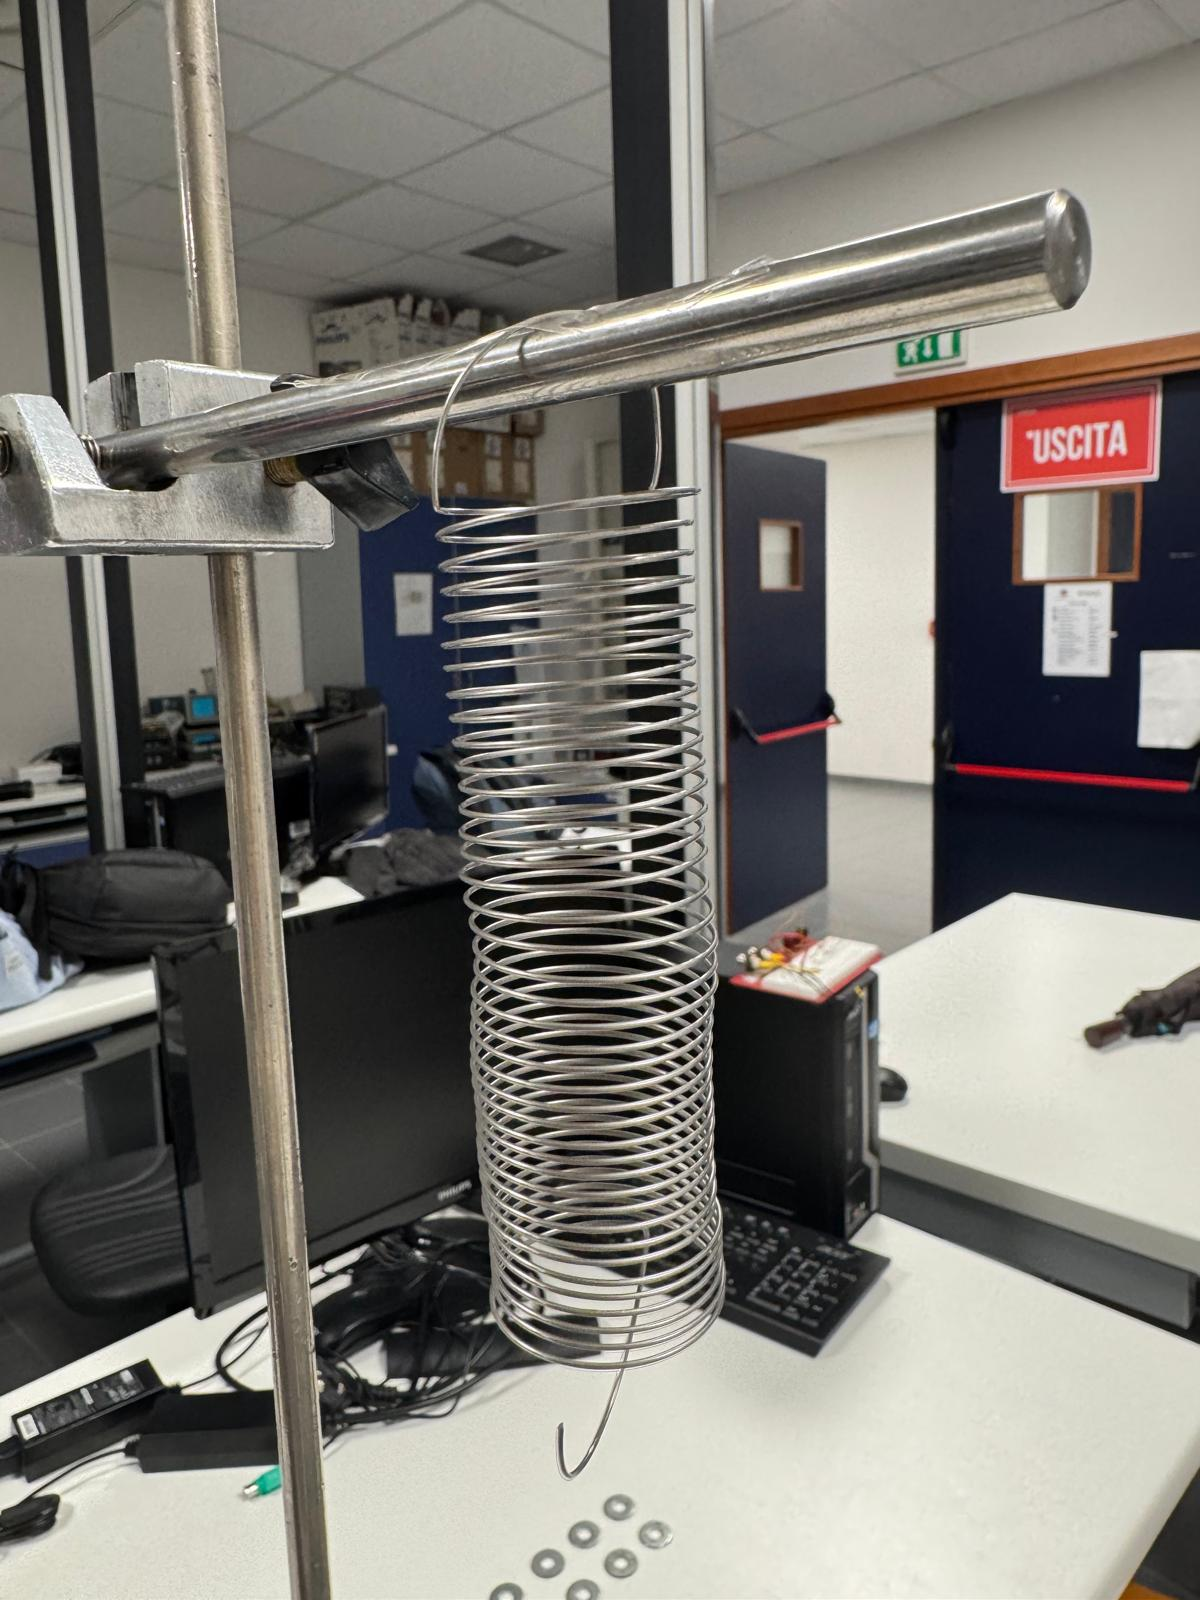
\includegraphics[width=0.55\textwidth]{molla.jpg}
  \caption{Molla utilizzata in laboratorio posta sul relativo supporto.}
\end{figure}
\begin{figure}[H]
  \centering
  \subfloat[Supporto per rondelle e rondelle utilizzate in laboratorio.]{%
    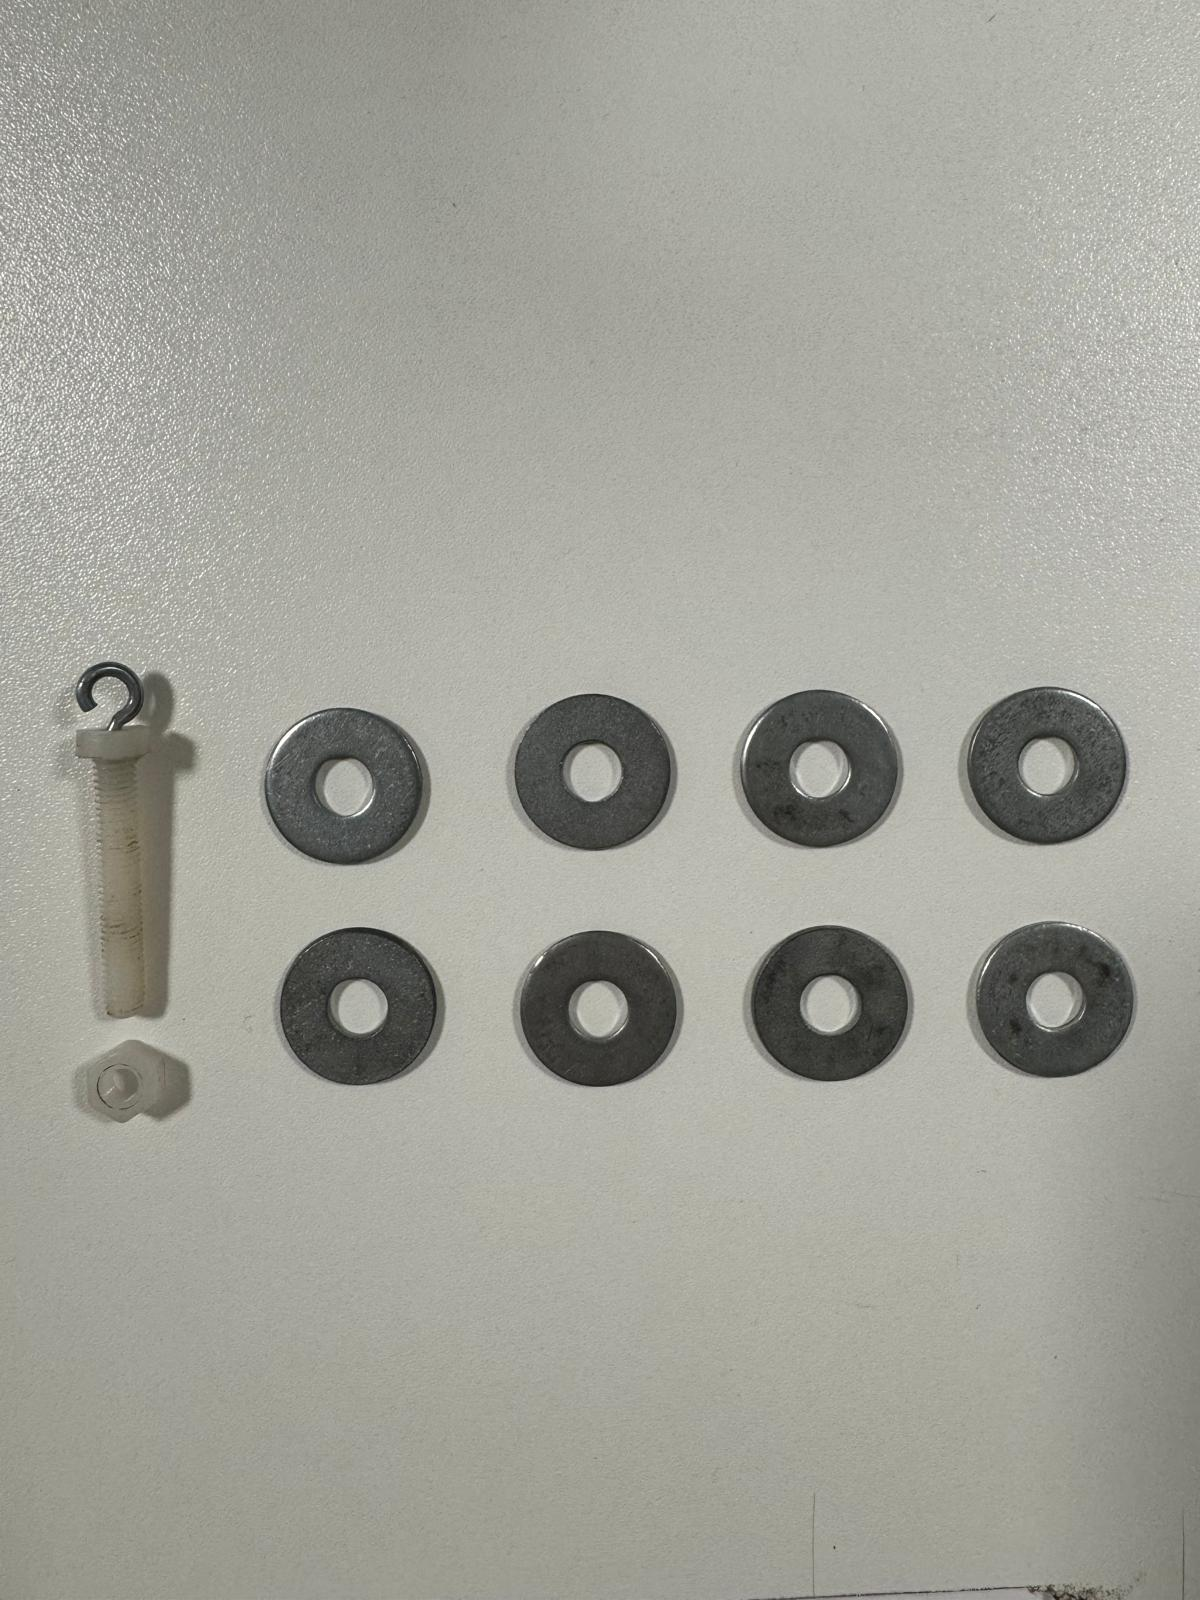
\includegraphics[width=0.35\textwidth]{supportorondelle.jpg}
  }
  \hspace{0.5cm} % Spazio tra le due immagini
  \subfloat[Metro a nastro utilizzato in laboratorio.]{%
    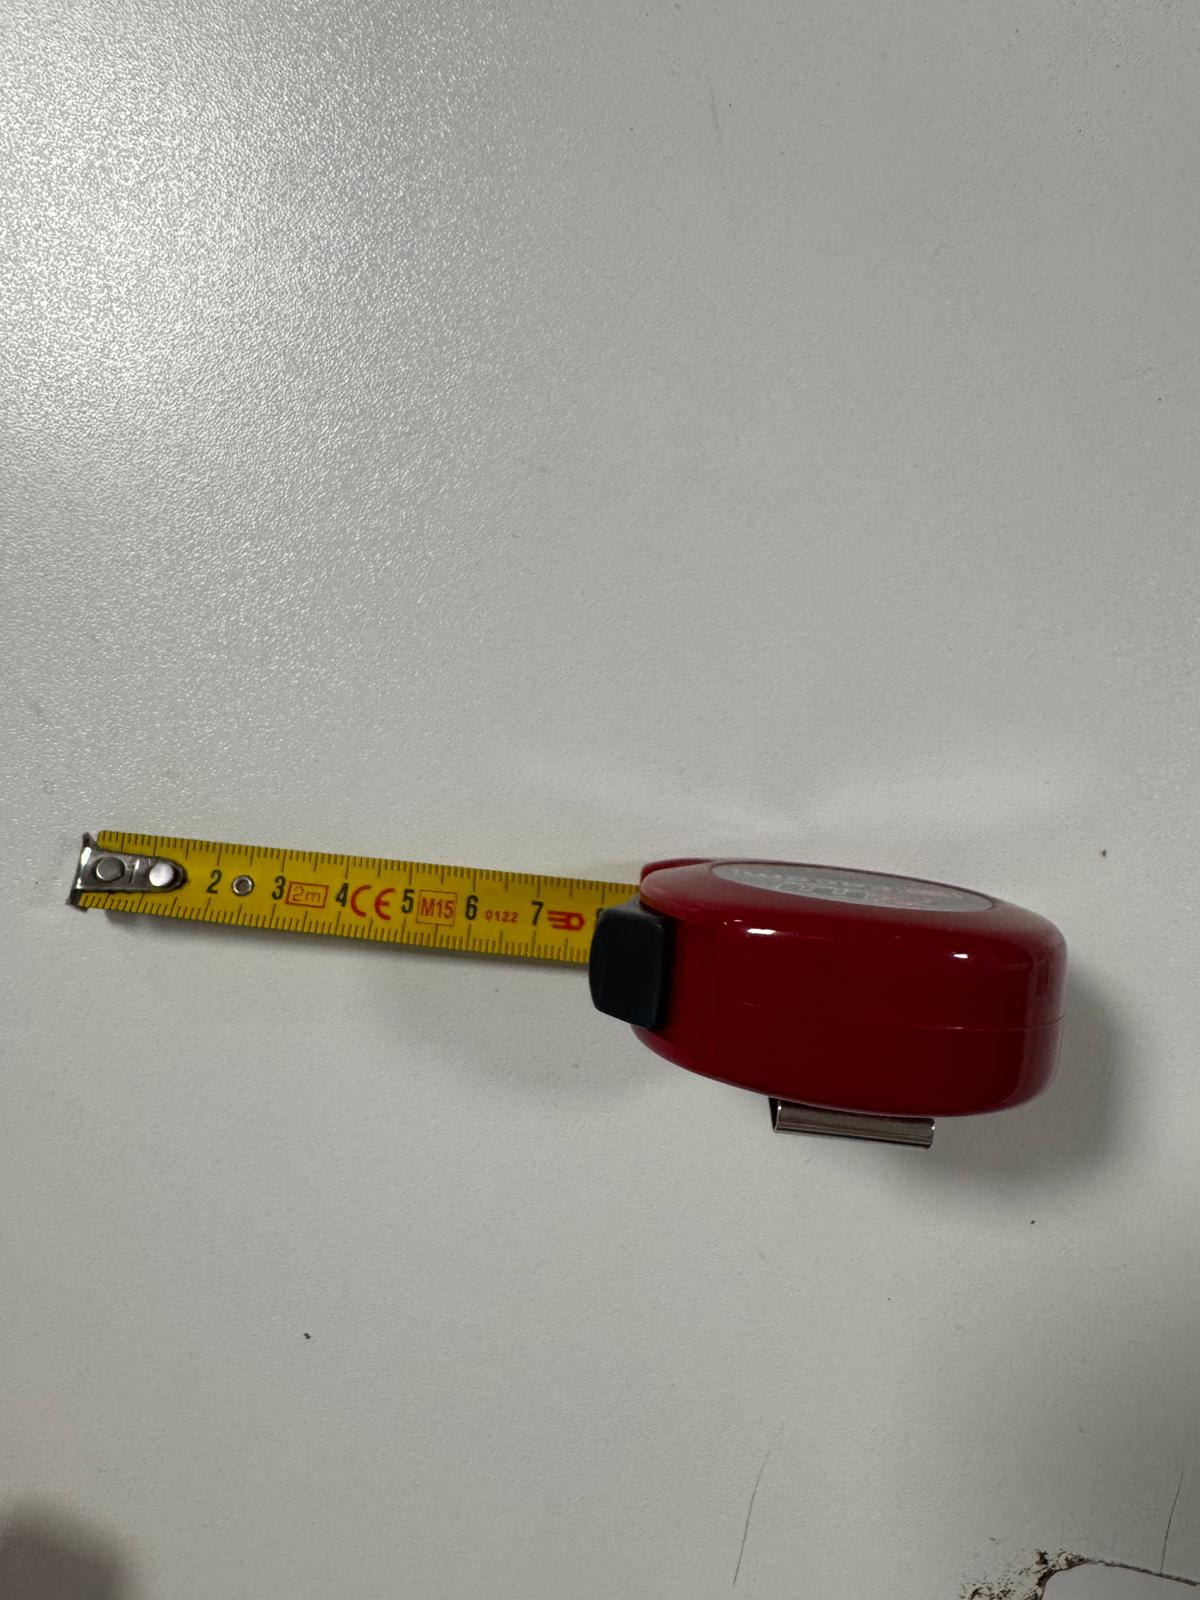
\includegraphics[width=0.35\textwidth]{metro.jpg}
  }
  \label{fig:due_immagini}
\end{figure}

%%%%%%%%%%%%%%%%%%%%%%%%%%%%%%%%%%%%%%%%%%%%%%%%%%
% DESCRIZIONE E ANALISI DEI DATI SPERIMENTALI
%%%%%%%%%%%%%%%%%%%%%%%%%%%%%%%%%%%%%%%%%%%%%%%%%%
\section{Descrizione e analisi dei dati spereimentali}
\subsection{Metodo Statico}

La lunghezza della molla a riposo è: $l_{riposo}= (11\pm 0.05)\ cm$. La forza stimata a per raddoppiare la lunghezza è di circa $F_{max}= 0.4291\ N$. Le diverse masse $M$ prese in considerazione saranno tali da ottenere un allungamento $\Delta x \in[0, 11]\ cm$. Abbiamo quindi effettuato $10$ misurazioni di massa ma solo le prime $8$ sono state utilizzate per misurare l'allungamento della molla poichè le altre sforano l'intervallo prestabilito. In realtà $\Delta x_7$ e $\Delta x_8$ non rientrano nell'intervallo ma sono state prese in considerazione poichè il numero minimo di misurazioni da valutare è $8$.
\begin{table}[H]
\centering
\begin{tabular}{|c|c|}
\hline
\textbf{$M$ $[kg]$} & \textbf{$\Delta x$ $[m]$} \\
\hline
$0.00758\pm 0.00001$ & $0.024\pm 0.0005$ \\
$0.01272\pm 0.00001$ & $0.04\pm 0.0005$ \\
$0.01786\pm 0.00001$ & $0.057\pm 0.0005$ \\
$0.02301\pm 0.00001$ & $0.0735\pm 0.0005$ \\
$0.02813\pm 0.00001$ & $0.093\pm 0.0005$ \\
$0.03330\pm 0.00001$ & $0.01085\pm 0.0005$ \\
$0.03853\pm 0.00001$ & $0.0126\pm 0.0005$ \\
$0.04374\pm 0.00001$ & $0.0143\pm 0.0005$ \\
\hline
\end{tabular}
\caption{La tabella mette in relazione l'allungamento della molla $\Delta x$ in corrispondenza della massa $M$}
\label{tab:}
\end{table}

\begin{figure}[H]
  \centering
  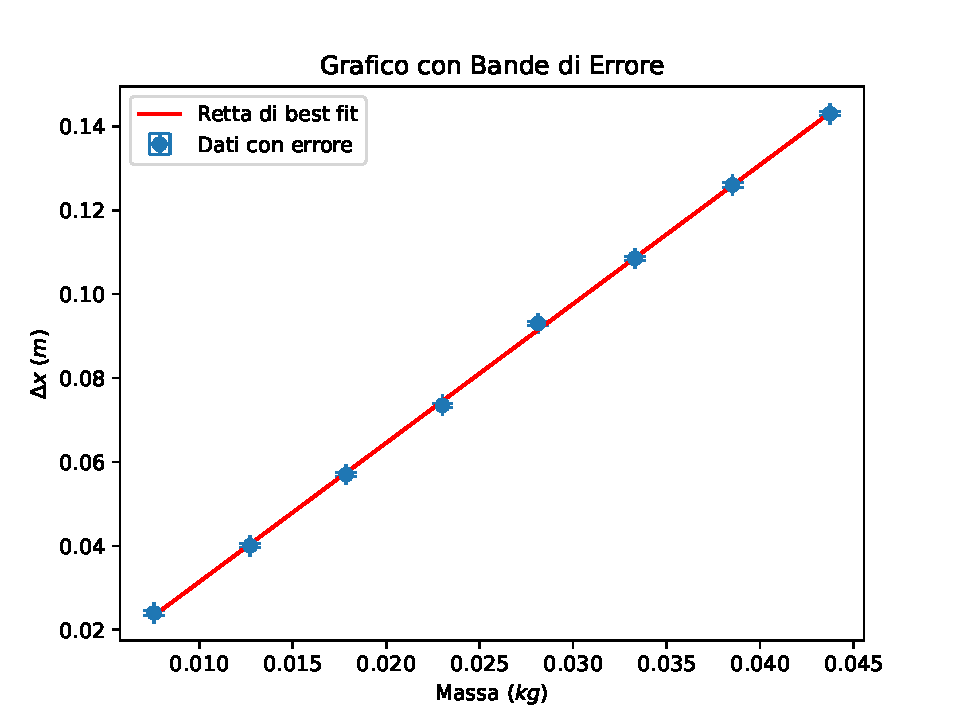
\includegraphics[width=1\textwidth]{grafico1p1.pdf}
  \caption{Grafico dell'allungamento della molla in funzione della massa. Valori in Tabella (2). \\
    Coefficiente angolare = ($3.31398\pm 0.07458$) $\frac{m}{kg}$ (Vedi Legge (10) e (12)).}
\end{figure}
Dalla Legge (1) sappiamo che il coefficiente angolare $b$ della retta dei minimi quadrati è legato alla costante elastica $k$ dalla relazione:
\begin{equation}
    b=\frac{g}{k}
\end{equation}
E quindi, considerando la propagazione dell'errore di $b$ su $k$, otteniamo:
%%%%%%%%%%%%%%%%%%%%%%%%%%%%%%%%%%%%%%%%%%%%%%%%%%
%%%%%%%%%%%%%%%%%%%%%%%%%%%%%%%%%%%%%%%%%%%%%%%%%%
%%%%%%%%%%%%%%%%%%%%%%%%%%%%%%%%%%%%%%%%%%%%%%%%%%
% qui dovremmo riportare le stime e gli errori con al più 2 cifre significative
\begin{equation}
    k = (2.96 \pm 0.07)\ \frac{N}{m} 
\end{equation}
%%%%%%%%%%%%%%%%%%%%%%%%%%%%%%%%%%%%%%%%%%%%%%%%%%
%%%%%%%%%%%%%%%%%%%%%%%%%%%%%%%%%%%%%%%%%%%%%%%%%%
%%%%%%%%%%%%%%%%%%%%%%%%%%%%%%%%%%%%%%%%%%%%%%%%%%

\subsection{Metodo Dinamico}
Per ognuna delle masse in Tabella (2) è stato misurato il tempo di dieci oscillazioni della molla. Questa misurazione è stata effettuata cinque volte per ognuna delle masse.
\begin{table}[H]
\centering
\begin{tabular}{|c|c|c|c|c|c|}
\hline
\textbf{$M$ $[kg]$} & \textbf{$t_1$ $[s]$} & \textbf{$t_2$ $[s]$} & \textbf{$t_3$ $[s]$} & \textbf{$t_4$ $[s]$} & \textbf{$t_5$ $[s]$} \\
\hline
$0.00758\pm 0.00001$ & $3.95\pm 0.01$ & $4.05\pm 0.01$ & $3.83\pm 0.01$ & $3.80\pm 0.01$ & $4.05\pm 0.01$ \\
$0.01272\pm 0.00001$ & $4.52\pm 0.01$ & $4.71\pm 0.01$ & $4.88\pm 0.01$ & $4.58\pm 0.01$ & $4.62\pm 0.01$ \\
$0.01786\pm 0.00001$ & $5.41\pm 0.01$ & $5.53\pm 0.01$ & $5.57\pm 0.01$ & $5.34\pm 0.01$ & $5.24\pm 0.01$ \\
$0.02301\pm 0.00001$ & $5.95\pm 0.01$ & $6.05\pm 0.01$ & $5.95\pm 0.01$ & $6.01\pm 0.01$ & $6.08\pm 0.01$ \\
$0.02813\pm 0.00001$ & $6.68\pm 0.01$ & $6.85\pm 0.01$ & $6.55\pm 0.01$ & $6.84\pm 0.01$ & $6.57\pm 0.01$ \\
$0.03330\pm 0.00001$ & $7.14\pm 0.01$ & $7.40\pm 0.01$ & $7.13\pm 0.01$ & $7.17\pm 0.01$ & $6.99\pm 0.01$ \\
$0.03853\pm 0.00001$ & $7.55\pm 0.01$ & $7.80\pm 0.01$ & $7.53\pm 0.01$ & $7.80\pm 0.01$ & $7.87\pm 0.01$ \\
$0.04374\pm 0.00001$ & $7.89\pm 0.01$ & $8.08\pm 0.01$ & $7.87\pm 0.01$ & $8.16\pm 0.01$ & $7.75\pm 0.01$ \\
\hline
\end{tabular}
\caption{La tabella contiene le cinque misurazioni delle dieci oscillazioni della molla per ogni massa $M$ utilizzata.}
\label{tab:}
\end{table}
Da questa tabella è stato poi calcolato il periodo di oscillazione di ognuna delle masse. Il valore assoluto è dato dalla media delle cinque misurazioni, l'incertezza è stata calcolata per semidispersione.
\begin{table}[H]
\centering
\begin{tabular}{|c|c|}
\hline
\textbf{$M$ $[kg]$} & \textbf{$T$ $[s]$} \\
\hline
$0.00758\pm 0.00001$ & $0.39\pm 0.02$ \\
$0.01272\pm 0.00001$ & $0.47\pm 0.02$ \\
$0.01786\pm 0.00001$ & $0.54\pm 0.02$ \\
$0.02301\pm 0.00001$ & $0.60\pm 0.01$ \\
$0.02813\pm 0.00001$ & $0.67\pm 0.01$ \\
$0.03330\pm 0.00001$ & $0.72\pm 0.02$ \\
$0.03853\pm 0.00001$ & $0.77\pm 0.02$ \\
$0.04374\pm 0.00001$ & $0.80\pm 0.02$ \\
\hline
\end{tabular}
\caption{La tabella mette in relazione la massa $M$ agganciata alla molla in corrispondenza del periodo di oscillazione $T$}
\label{tab:}
\end{table}
\begin{figure}[H]
  \centering
  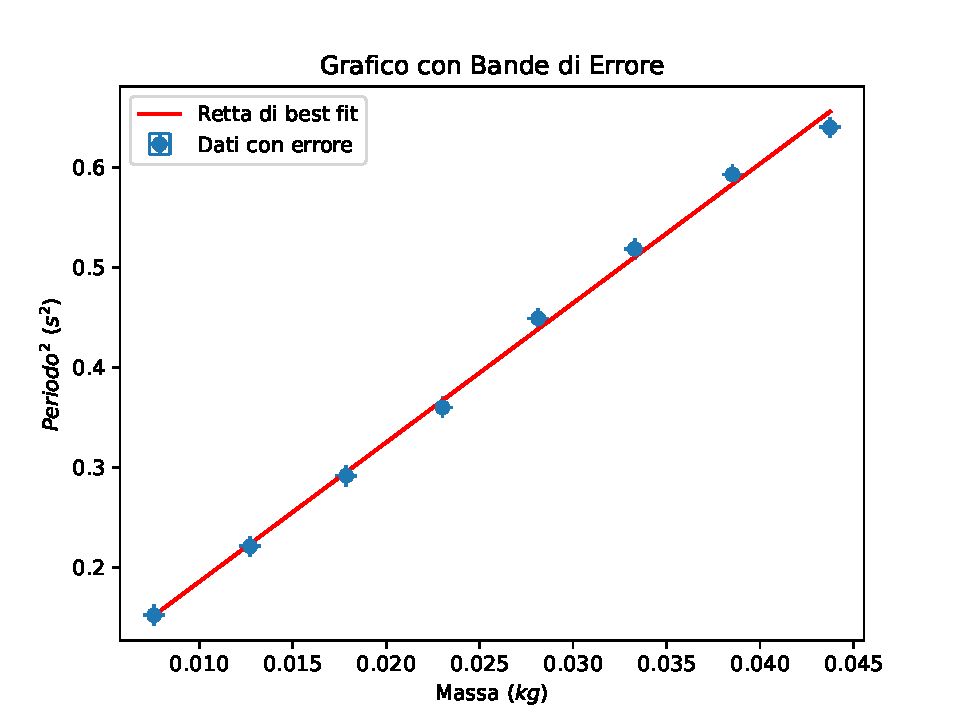
\includegraphics[width=1\textwidth]{grafico1p2.pdf}
  \caption{Grafico del quadrato del periodo di oscillazione della molla in funzione della massa. Valori in Tabella (4). \\
    Coefficiente angolare = ($13.93857\pm 0.88895$) $\frac{m}{N}$ (Vedi Legge (10) e (12)).}
\end{figure}
Utilizzando la Legge (7) e considerando anche la massa della molla $m = (15.45\pm 0.01)\ g$ otteniamo esattamente lo stesso coefficiente angolare riportato in Figura (3). Ne consegue che la massa della molla è trascurabile. La stima del coefficiente angolare e dell'intercetta delle rette di best fit è stata effettuata utilizzando il metodo dei minimi quadrati.
Siano $b$ il coefficiente angolare e $a$ l'intercetta della retta:
\begin{equation}
    b=\frac{\displaystyle\sum_{i=1}^{N}[(x_i-\overline{x})(y_i-\overline{y})]}{\displaystyle\sum_{i=1}^{N}(x_i-\overline{x})^2}
\end{equation}
\begin{equation}
    a=\overline{y}-b\overline{x}
\end{equation}
Con $\overline{x}=\frac{\displaystyle\sum_{i=1}^{N}x_i}{N}$ e $\overline{y}=\frac{\displaystyle\sum_{i=1}^{N}y_i}{N}$
mentre le incertezze:
\begin{equation}
    \Delta b=3\sigma_b
\end{equation}
\begin{equation}
    \Delta a=3\sigma_a
\end{equation}
Con
\begin{equation}
    \sigma_b=\sigma_y\sqrt{\frac{N}{\Delta}}
\end{equation}
\begin{equation}
    \sigma_y=\sqrt{\frac{\displaystyle\sum_{i=1}^{N}(y_i-bx_i-a)^2}{N-2}}
\end{equation}
\begin{equation}
    \sigma_a=\sigma_y\sqrt{\frac{\displaystyle\sum_{i=1}^{N}x_i^2}{\Delta}}
\end{equation}
\begin{equation}
    \Delta=N\displaystyle\sum_{i=1}^{N}(x_i-\overline{x})^2
\end{equation}
Conoscendo il coefficiente angolare della retta di regressione si ricava facilmente il valore della costante elastica della molla. Infatti, dalla relazione:
\begin{equation}
    T^2=\frac{4\pi^2}{k}M
\end{equation}
Ricaviamo la costante $k$ come:
\begin{equation}
    k=\frac{4\pi^2}{b}
\end{equation}
E l'incertezza assoluta $\Delta k$:
\begin{equation}
    \Delta k=\frac{\Delta b}{b}k
\end{equation}
Quindi otteniamo il valore $k$:
%%%%%%%%%%%%%%%%%%%%%%%%%%%%%%%%%%%%%%%%%%%%%%%%%%
%%%%%%%%%%%%%%%%%%%%%%%%%%%%%%%%%%%%%%%%%%%%%%%%%%
%%%%%%%%%%%%%%%%%%%%%%%%%%%%%%%%%%%%%%%%%%%%%%%%%%
% cifre significative
\begin{equation}
    k = (2.83 \pm 0.18)\ \frac{N}{m} 
\end{equation}
%%%%%%%%%%%%%%%%%%%%%%%%%%%%%%%%%%%%%%%%%%%%%%%%%%
%%%%%%%%%%%%%%%%%%%%%%%%%%%%%%%%%%%%%%%%%%%%%%%%%%
%%%%%%%%%%%%%%%%%%%%%%%%%%%%%%%%%%%%%%%%%%%%%%%%%%

\section{Conclusioni }
I due approcci conducono a risultati compatibili. La discrepanza tra i due valori è inferiore alla somma degli errori assoluti:
\begin{center}
    |2.96 - 2.83| = 0.13 < 0.07 + 0.18
\end{center}

\end{document}